\section{Results}







% Original images, adversarial images, and corresponding adversarial noise created with FGSM ( ϵ=0.02) in different black-box settings


\subsection{Efficiency analysis}


\begin{figure*}[h!]
     \centering
     \begin{subfigure}
         \centering
         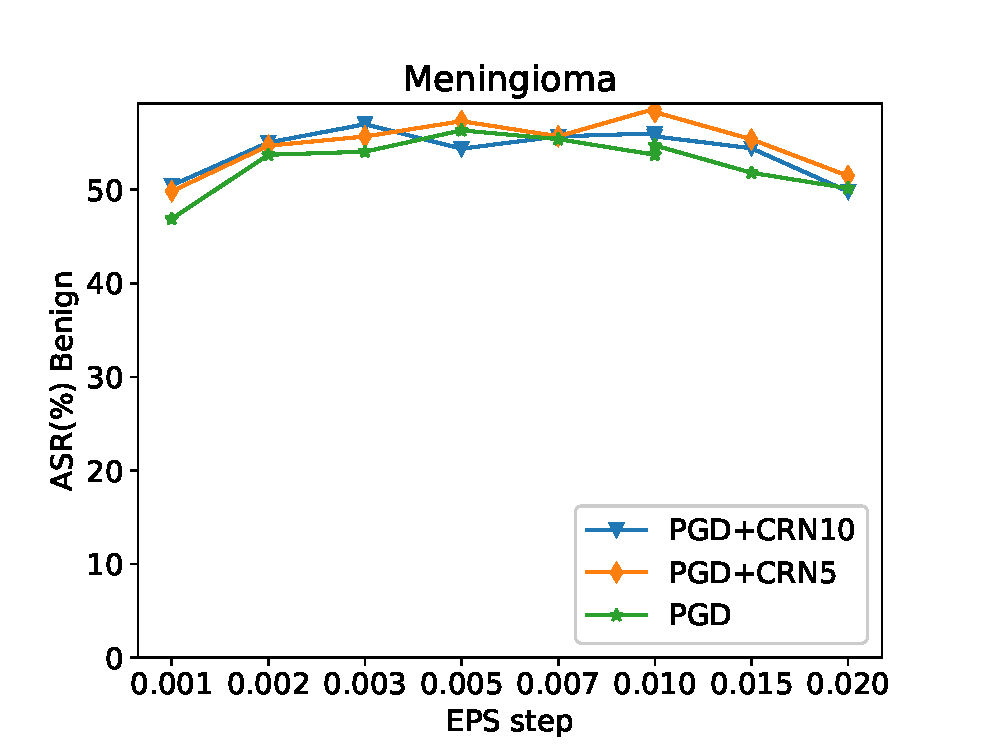
\includegraphics[width=0.32\textwidth]{Meningioma_ASR_EPS_steps.eps}
          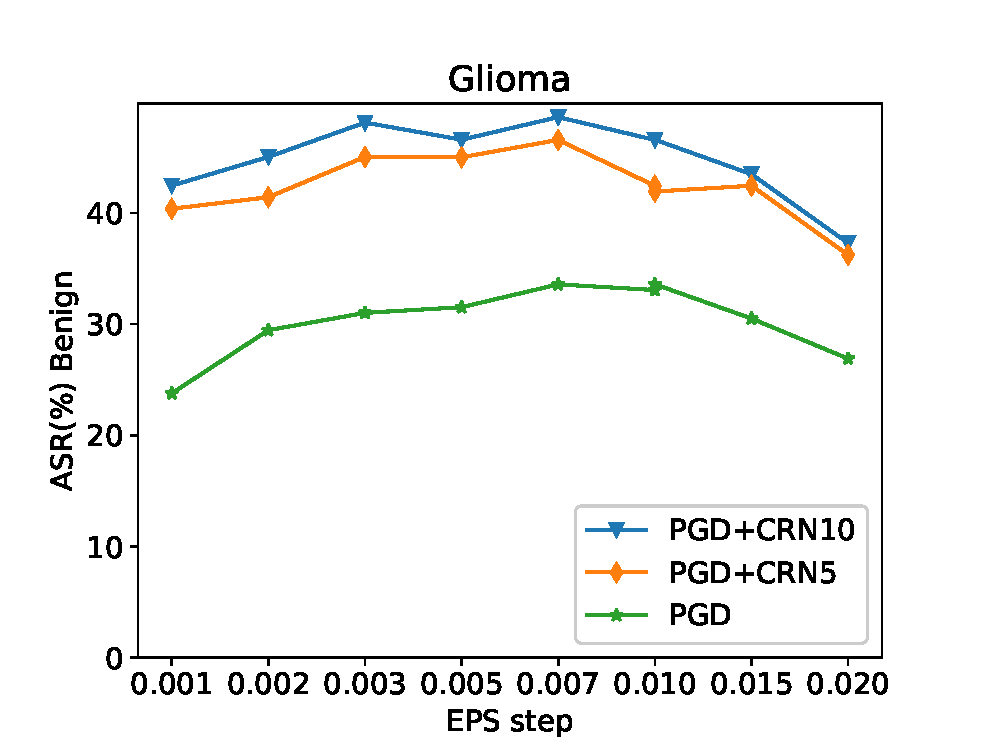
\includegraphics[width=0.32\textwidth]{Glioma_ASR_EPS_steps.eps}
           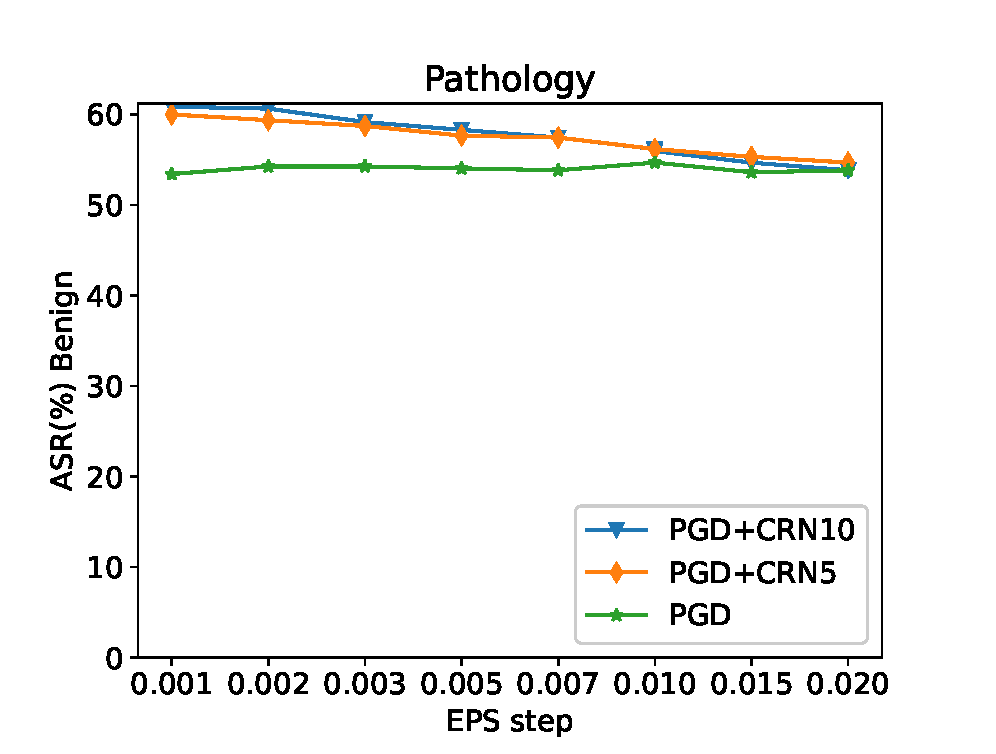
\includegraphics[width=0.32\textwidth]{Pathology_ASR_EPS_steps.eps}
         \caption{Average ASR on benign clients }
         \label{fig:y equals x}
     \end{subfigure}
     \hfill
     \begin{subfigure}
          \centering
         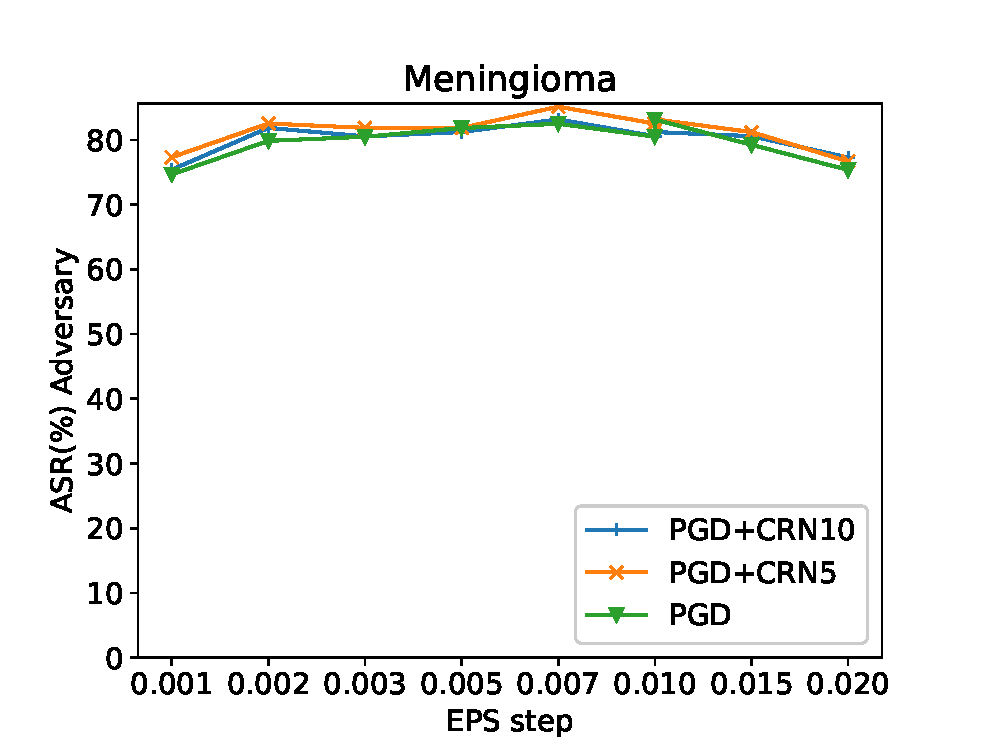
\includegraphics[width=0.32\textwidth]{Meningioma_others_EPS_steps.eps}
          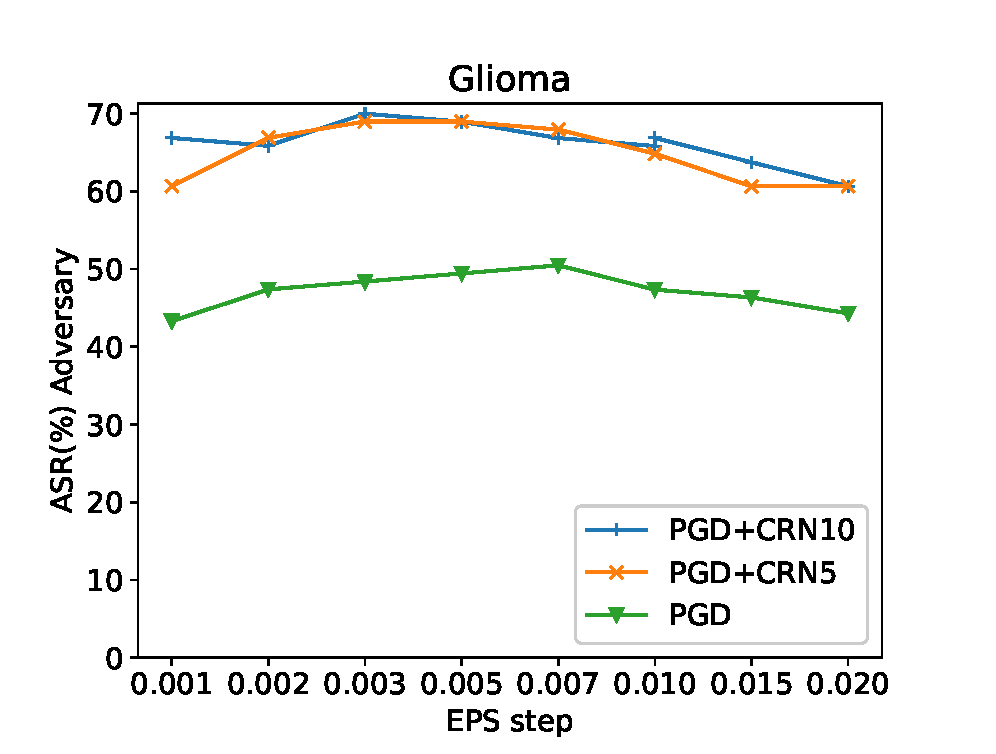
\includegraphics[width=0.32\textwidth]{Glioma_others_EPS_steps.eps}
           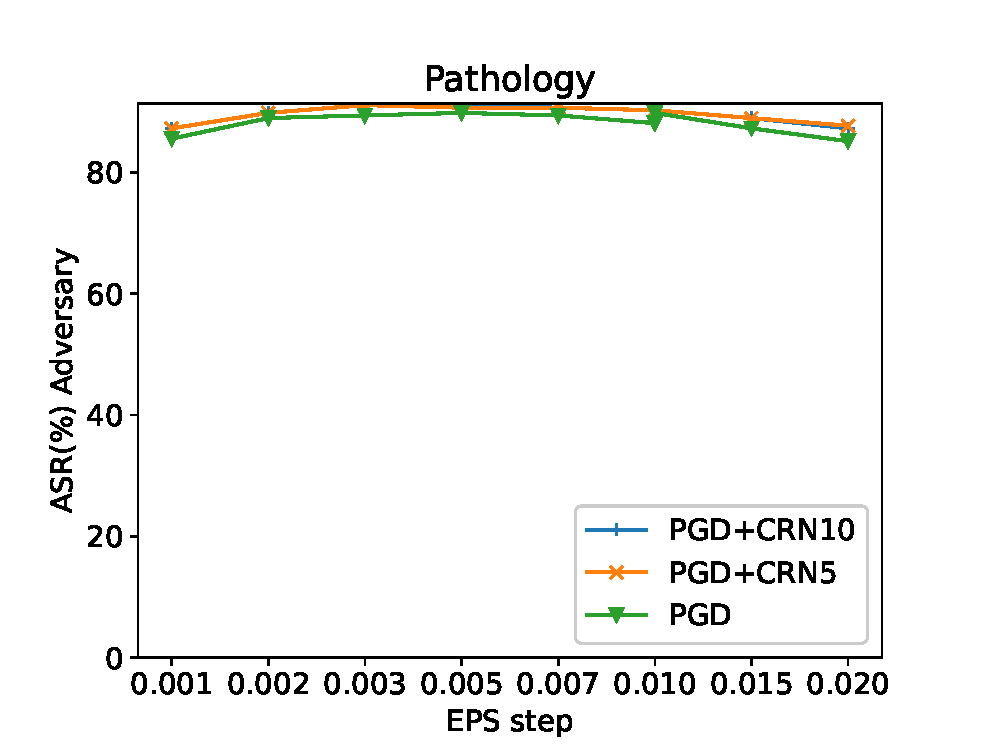
\includegraphics[width=0.32\textwidth]{Pathology_others_EPS_steps.eps}
         \caption{Average ASR on advesarial client }
         \label{fig:y equals x}
     \end{subfigure}
     \hfill
        \caption{Effect of Error perturbation step $\alpha$ on attack transferability. PGD attack with CRN initalizations used 10 models and another one loading 5. ASR is calculated on benign and adversary clients. The results of with varying perturbation steps. The higher ASR on benign clients shows higher transferability}
        \label{fig:three graphs}
\end{figure*}

The models are trained in an FL enviroment. Average test results, or clean accuracy shows the average performance of clients on unperturbed test data. This could be a baseline for comparison of attacks.
Here we compare the computational complexity of iterative algorithms. The comparison is based on the time required to train one batch of adversarial examples, with  $\epsilon=0.05$ and $\alpha=0.001$. The average Attack success rate is the average of ASR for all test samples of all clients and indicates the transferability in the FL network.
As expected \ref{table_time}, the higher iteration rounds take more computation and lead to higher AASR. Generally, computational complexity has a linear dependence on the number of iterations. However, the increase in transferability can vary. If PGD performs poorly initially, having higher iterations doesn't help much. 

Also, CRN does not require additional computation. Similar to single-step methods, computational load is small but increases on high-resolution images. As an example, the pathology dataset requires more calculation than MRI data. 
However, the overall time is far less than iterative models, and also it could enhance the transferability much better. The effect is consistent among different datasets. 
% However,  This means that Pathology images have better AASR than MRI images in baseline and CRN enabled attacks.
% Also,  

% PGD can sometimes perform poorly, even in higher iterations. Enabling the initialization might  


\begin{table}[h!]
\centering
\setlength{\tabcolsep}{6pt}
\renewcommand\arraystretch{1.22}
\caption{ \small Comparison of iterative models and their copmutational efficiency, on performing computations on one batch of data.  ACC shows average client performance for unperturbed test data. AASR is average ASR on all clients.}
\begin{tabular}{| *{5}{c|} }
\hline
Dataset  & Attack type & ACC & AASR & time (sec)
\\   \hline  
\multirow{3}{5em}{Meningioma}     &\textbf{PGD-1+CRN10}&\multirow{3}{3em}{84.12\%}&\textbf{63.92\%} & \textbf{0.217}  \\
 &PGD-20&&27.52\% & 3.423 \\
&PGD-40&&32.99\% & 6.794  \\ \hline
\multirow{3}{4em}{Pathology}     &\textbf{PGD-1+CRN10}&\multirow{3}{3em}{77.01\%}&\textbf{90.92\%} & \textbf{0.354} \\
&PGD-20&&60.98\% & 5.464\\
&PGD-40&&82.27\% & 10.843 \\ \hline
\multirow{3}{3em}{Glioma}     &\textbf{PGD-1+CRN10}&\multirow{3}{3em}{61.84\%}&\textbf{70.55}\% & \textbf{0.216}  \\
&PGD-20&&51.83\% &3.420  \\
&PGD-40&&63.77\% & 6.793  \\ \hline


\end{tabular}
\label{table_time} 
\end{table}




\subsection{Effect perturbation degree}

We performed attack scenarios to evaluate the effect of perturbation degree $\epsilon$  on attack success on the model. We compared the baseline attack to CRN- enabled attacks. ASR is calculated on benign and adversary clients and is shown in Fig \ref{fig: epsilon graphs}.

More successful attacks on adversaries led to higher transferability to benign clients. Low values of $\epsilon$ can decrease transferability to a large extent. $\epsilon$ = 0.01 has poor performance on all the clients. Generally, Higher $\epsilon$ values lead to higher ASR in all scenarios. Although for Meningioma and Glioma images, increasing $\epsilon$ from 0.04 didn't have much positive effect in PGD and FGSM methods on the adversarial client. 
In pathology images, Iterative models can reach perfect accuracy on the adversarial client and have very high transferability.

CRN  has a positive effect on transferability in all scenarios. Also, CRN-enabled models are more dependent on $\epsilon$; their extent can vary depending on the dataset, attack method, and value of $\epsilon$.
Tuning $\epsilon$  might be tricky since performance and imperceptibility should be considered together.High $\epsilon$ values mean more distortion in the image. We performed an FGSM attack with varying $\epsilon$ values to evaluate the perturbation effect visually. Fig \ref{fig:perturbedMRI} shows the results of perturbed images with different perturbation degrees and their comparison with the unperturbed image. Note that perturbation values below  $\epsilon=0.05$ cause limited distortion.


Iterative models can reach high ASR very quickly with increasing $\epsilon$. 

\begin{figure*}[h!]
 \centering
 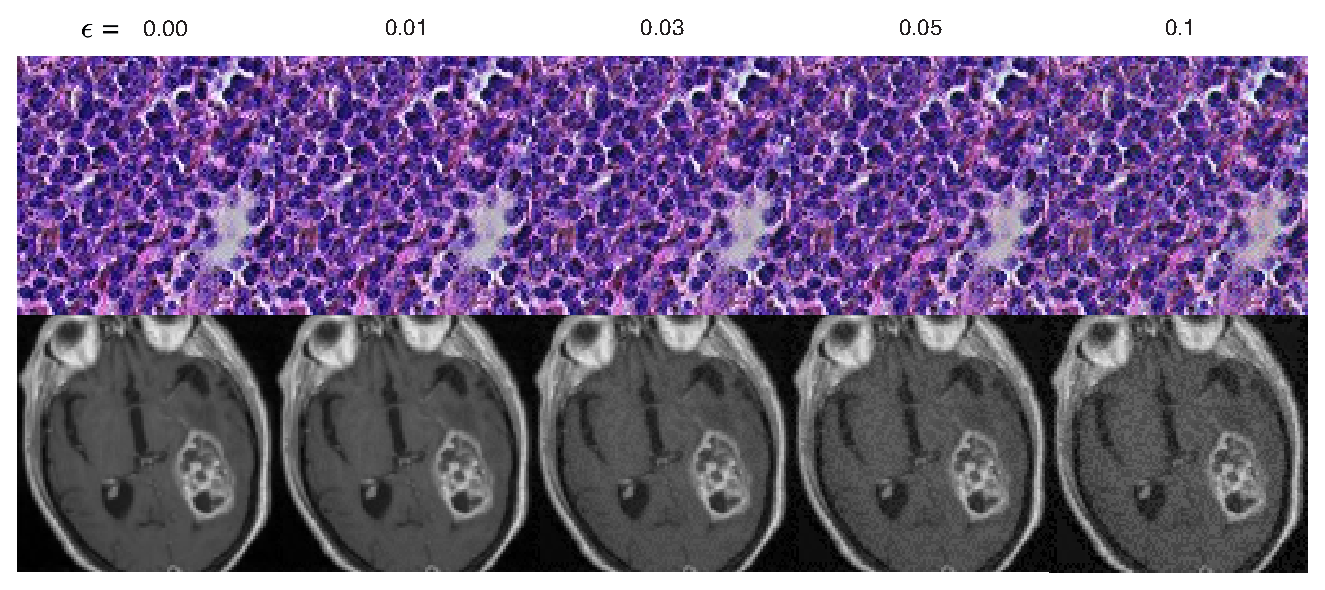
\includegraphics[width=0.8\textwidth]{Adversarial_attacks-5.eps}
 \caption{\small From (a) to (f), normal tumor image, and petrurbed images with FGSM attack, with perturbation parameters: $\epsilon$ = 0.01, 0.03, 0.05,  0.10, respectively}
 \label{fig:perturbedMRI}
\end{figure*}











% \subsection{AATR}
% \begin{table}[h]
% \centering
% \setlength{\tabcolsep}{8pt}
% \renewcommand\arraystretch{1.4}
% \caption{Result of our experiments for PGD attack on Pathology data $\epsilon$ values. The iterative models are trained for 40 rounds with step size of 0.01. \hl{\faQuestion maybe you can change the word for without CRN}}
% % \begin{tabular}{cccccccccccc}
% \begin{tabular}{| *{4}{c|} }\hline
% % Dataset  & Attack type & \multicolumn{2}{c|}{ $\epsilon=0.01$} & \multicolumn{2}{c|}{ $\epsilon=0.03$}           &    \multicolumn{2}{c|}{ $\epsilon=0.05$}    & \multicolumn{2}{c|}{ $\epsilon=0.07$}                                                              \\ \hline
%  Dataset&\multicolumn{3}{c|}{ FGSM}    
% %  &              \multicolumn{3}{c|}{ PGD}                                                                           \\  

%  \cline{2-5}
% &Baseline&CRN5 &CRN10\\\hline

% Meningioma&84.80\%&\textbf{86.31}\%&{84.02\%}
% % \%&83.73\%  &\textbf{84.25}\%  &84.16\%
% \\\hline
% Glioma&82.32\% &87.06\%&\textbf{89.98\%}
% % &74.89\%&\textbf{83.64}\% &82.32\%
% \\\hline

% Pathology&\textbf{90.67\%}&{84.81\%}\%&{85.98\%}
% % \%&79.86\% &86.79\%&\textbf{86.93\%}
% \\\hline



% \end{tabular}
% \label{table_core} 
% \end{table}










\subsection{Effect perturbation step}


Another critical parameter is the step of change in iterative methods. {$\alpha$} is shown to be highly deterministic in specific settings, but is not yet investigated in MIA domain. To evaluate how $\alpha$ can affect transferability, we examined the clients with $\eps=0.03$. Under various steps. The general observation is that there is an optimal middle range the same as $\epsilon$. The step size of 0.007 led to the highest transferability in MRI images. Larger steps led to a sharp decrease in transferability. For pathology images, midspans, about 0.007 led to the best ASR on the adversary, and higher values decreased both ASR on adversary and transferability. However, smaller steps also had high ASR values. 







\subsection{Error tranferability}




Another measure is the average error transfer rate (AETR). Although PGD outperforms FGSM in ASR, in AETR, the results are close. PGD is trained for 40 iterations, and the models are compared with and without CRN.
Both FGSM and PGD having high AETR suggest that although FGSM might not be able to produce high-quality samples in general, the good examples which can fool the adversary are also highly transferable to benign clients. And can be better than PGD samples. CRN generally increases the AETR. 




\begin{table*}[h!]
\centering
\setlength{\tabcolsep}{8pt}
\renewcommand\arraystretch{1.4}
\caption{Result of Average Error Transfer Rate (AETR) for FGSM and PGD methods, with and without CRN initalization }
% \begin{tabular}{cccccccccccc}
\begin{tabular}{| *{7}{c|} }\hline
% Dataset  & Attack type & \multicolumn{2}{c|}{ $\epsilon=0.01$} & \multicolumn{2}{c|}{ $\epsilon=0.03$}           &    \multicolumn{2}{c|}{ $\epsilon=0.05$}    & \multicolumn{2}{c|}{ $\epsilon=0.07$}                                                              \\ \hline
 Dataset&\multicolumn{3}{c|}{ FGSM}     &              \multicolumn{3}{c|}{ PGD}                                                                           \\  

 \cline{2-7}
&Baseline&CRN5 &CRN10&Baeline&CRN5&CRN10\\\hline

Meningioma&84.80\%&\textbf{86.31}\%&{84.02}\%&83.73\%  &\textbf{84.25}\%  &84.16\%\\\hline
Glioma&82.32\% &87.06&\textbf{89.98}&74.89\%&\textbf{83.64}\% &82.32\%\\\hline

Pathology&\textbf{90.67\%}&{84.81}\%&{85.98}\%&79.86\% &86.79\%&\textbf{86.93\%}\\\hline



\end{tabular}
\label{table_core} 
\end{table*}

